\documentclass[10pt,twocolumn,letterpaper]{article}
\usepackage[margin=0.62in,columnsep=0.2in]{geometry}
\usepackage{times}
\usepackage[T1]{fontenc}
\usepackage{graphicx,booktabs,array,enumitem,titlesec,caption,amsmath}
\usepackage[hidelinks]{hyperref}
\setlist{nosep,leftmargin=1.1em}
\renewcommand{\thesection}{\Roman{section}}\renewcommand{\thesubsection}{\Alph{subsection}}
\titleformat{\section}{\normalsize\bfseries\scshape\centering}{\thesection.}{0.5em}{}
\titleformat{\subsection}{\normalsize\itshape}{\thesubsection.}{0.5em}{}
\titlespacing*{\section}{0pt}{6pt}{3pt}
\titlespacing*{\subsection}{0pt}{4pt}{2pt}
\captionsetup{font=small,labelfont=bf,skip=3pt}
\setlength{\textfloatsep}{6pt}\setlength{\dbltextfloatsep}{6pt}\setlength{\floatsep}{5pt}
\setlength{\parskip}{1pt}
\raggedbottom
\newcommand{\code}[1]{\texttt{\small #1}}

\title{\vspace{-1.6em}\Large\bfseries CS471 Status Report:\\ Making Local Quantized LLMs More Energy Efficient\vspace{-0.6em}}
\author{Mihai Indreias \qquad Filip Corlan\\ \small EPFL, Lausanne, Switzerland}
\date{\vspace{-1.2em}}

\begin{document}
\maketitle

\section{Response to Proposal Feedback}

\subsection{Share of linear layers in GPU time}
\begin{quote}\small
``Your hypothesis is that linear layers are 30\% of GPU execution time, but you do not provide any insights to
support this claim.''
\end{quote}
The 30\% figure in the proposal was a rough estimate, and we have now measured it. We ran our target model,
Qwen3.8-27B in the quantized version UD-Q4\_K\_M, on an NVIDIA H100 GPU and recorded how long the GPU spends on each
kind of operation. An LLM works in two phases: it first reads the user's prompt (prefill), and then generates the
answer one token at a time (decode). Matrix multiplications with the model's weights take 84\% of GPU time in decode
and 76\% in prefill, so the hypothesis holds with a large margin.

\subsection{Choice of numerical formats}
\begin{quote}\small
``Half this report is explaining the numerical formats and lacks discussion on why these formats were
chosen\ldots\ Is it necessary to evaluate all these formats? Can preliminary experiments identify similar
architectural implications, so that findings generalize across groups of formats?''
\end{quote}
We study only the formats used by our target model
(Table~\ref{tab:model}), which is distributed in GGUF, the format that most people use to run LLMs on their own
machines. These are therefore the formats that matter in practice for local inference, which processes one request
at a time and is limited by energy, exactly the setting we want to study.

It is not necessary to study every format separately. Our first measurements show that the formats fall into three
groups, according to the extra work needed to decompress them rather than according to their size: formats with a
single scale per block, formats with two levels of scales and offsets (the ``K'' formats), and formats that look up
values in a small table (the ``IQ'' formats). Formats in the same group behave similarly, so we reason about these
three groups and expect our findings to carry over to other formats in each group.

For background, GGUF is the file format of llama.cpp, the engine behind most tools for running LLMs locally. A GGUF
file stores the weights of a model in compressed form. Each weight matrix is split into small blocks of 32 or 256
weights. Every weight in a block is stored as a small integer of 2 to 8 bits, and the block also stores a shared
scale factor (and in some formats an offset) that converts these integers back into real values. The formats
differ in how many bits they use and in how the scales are organized, and a single model usually mixes several of
them, using more bits for the weights that matter most for accuracy.

\begin{table}[t]
\centering\small
\caption{The weight formats used by our model, the group each belongs to, and their share of the data read and of
the GPU time spent while generating text.}
\label{tab:model}
\begin{tabular}{@{}llrr@{}}
\toprule
Format & Group & Share of data & Share of time\\
\midrule
IQ4\_XS & Lookup table & 37\% & 29\%\\
Q5\_K & Two-level & 34\% & 26\%\\
Q4\_K & Two-level & 16\% & 14\%\\
Q6\_K & Two-level & 9\% & 6\%\\
IQ4\_NL & Lookup table & 3\% & 2\%\\
Q8\_0 & Single scale & 0.5\% & 5\%\\
\bottomrule
\end{tabular}
\end{table}

\section{Update on Problem Definition}

The problem we study has changed since the proposal. The proposal asked whether hardware support for compressed
formats, as in the Avant-Garde design~\cite{ag}, makes LLMs run faster. Our measurements show that speed is the
wrong goal for local inference. To generate each token, the GPU must read every weight of the model from memory once
(15.5\,GB for our model), so the speed is limited by how fast memory can deliver data, not by how fast the GPU can
compute~\cite{splitwise}. Faster arithmetic would not help.

We therefore look at energy instead. Compressing the weights reduces the amount of data read from memory, and
moving data is the main source of energy use in computer chips~\cite{horowitz}. However, no GPU can read these
formats directly, so the GPU has to decompress every weight in software before using it, and this costs energy too.
We found that this cost is large: the most common format makes the weights 3.6 times smaller than uncompressed
16-bit weights, but reduces energy by only 2.2 times. Our new question is how much energy is spent on this software
decompression, and how much of it a small dedicated hardware unit could save.

\section{Update on Design Space}

\subsection{New dimensions}
Our new focus adds five dimensions to the design space. Table~\ref{tab:design} summarizes them by comparing the
choices made by Avant-Garde~\cite{ag} with ours.

\begin{table}[h]
\centering\small
\caption{New design dimensions, comparing Avant-Garde with our approach.}
\label{tab:design}
\begin{tabular}{@{}>{\raggedright\arraybackslash}p{0.27\columnwidth}>{\raggedright\arraybackslash}p{0.29\columnwidth}>{\raggedright\arraybackslash}p{0.36\columnwidth}@{}}
\toprule
Dimension & Avant-Garde & This project\\
\midrule
Part of the GPU & Matrix units & General-purpose cores\\\addlinespace[3pt]
Where weights are decompressed & Expanded in memory & Compressed until just before use\\\addlinespace[3pt]
How scales are applied & To every weight & Once per block\\\addlinespace[3pt]
Formats & Simple scales & Two-level scales, offsets, lookup tables\\\addlinespace[3pt]
Metric & Speed & Energy, total and above idle\\
\bottomrule
\end{tabular}
\end{table}

These choices follow from our setting. When generating text for a single user, the GPU uses its general-purpose
cores rather than the matrix units that Avant-Garde extends. Storing weights in expanded form roughly doubles the
data read from memory, which is exactly the cost we want to avoid, so we keep them compressed until the last
moment. Applying the scale once to the sum of each block, instead of to every weight, saves most of the
multiplications. GGUF needs more kinds of formats than Avant-Garde supports. Finally, a GPU uses a lot of power even
when idle, so a format that is processed more slowly also wastes idle energy, and we therefore report both the total
energy and the energy above idle.

\subsection{New related work}
Avant-Garde~\cite{ag} adds hardware support for simple compressed formats to a simulated GPU, but does not cover
the formats used by GGUF or the single-user setting. Other recent work designs hardware for similar block
formats~\cite{mxnpu} or for formats based on lookup tables~\cite{lut,flute}, and we will build on these.

\section{Questions, Hypotheses and Tests}

\subsection{Status of the proposal's questions}
We have answered the question of what limits LLM inference on the GPU: generating text is limited by reading weights
from memory, and matrix multiplications take most of the time, which confirms our original hypothesis. We have
partly answered how much the compressed formats cost, by measuring their energy on a single matrix. The question of
which hardware changes reduce this cost will be answered by our hardware design study. We have dropped the plan to
simulate Avant-Garde, because the available GPU power simulator is not accurate for modern GPUs, and we no longer
use speed as our main metric.

\subsection{New hypotheses}
\begin{itemize}
\item H1: Compressed formats cost more energy than the data they read would explain, and this extra energy, between
15\% and 40\%, comes from decompressing the weights in software.
\item H2: A hardware decompression unit costs only a small fraction of the energy of the arithmetic it feeds, so
formats that are complex for software are cheap for hardware.
\item H3: Adding such a unit would reduce the energy of generating text by more than 10\%.
\end{itemize}

\subsection{Methodology}
Our work has three parts. First, we measure energy on a real GPU. We run the matrix multiplications of each format
on the H100 while reading its built-in energy meter, and we compare formats that read the same amount of data but
need different amounts of decompression work. We then measure the energy of generating text with the full model.
Second, we design the hardware. We describe a small arithmetic unit in a hardware description language, starting
from a basic version without decompression and adding support for each group of formats in turn. We then use chip
design tools to estimate its area and power. Third, we combine the two. Because our design and the H100 use
different manufacturing technologies, we cannot compare their energy directly. Instead, we compare the extra energy
each one spends on decompression, relative to its own baseline.

\section{Results}
\label{sec:results}

\begin{table}[t]
\centering\small
\caption{How much smaller each format makes the weights, and how much it actually reduces energy, compared with
uncompressed 16-bit weights (F16). Measured on the H100 for one matrix multiplication.}
\label{tab:energy}
\begin{tabular}{@{}llrr@{}}
\toprule
Format & Group & Data reduction & Energy reduction\\
\midrule
F16 & Uncompressed & 1.00$\times$ & 1.00$\times$\\
Q8\_0 & Single scale & 1.88$\times$ & 1.65$\times$\\
Q4\_1 & Single scale & 3.20$\times$ & 2.69$\times$\\
Q4\_0 & Single scale & 3.56$\times$ & 2.65$\times$\\
IQ4\_NL & Lookup table & 3.56$\times$ & 2.37$\times$\\
IQ4\_XS & Lookup table & 3.76$\times$ & 2.52$\times$\\
Q6\_K & Two-level & 2.44$\times$ & 1.72$\times$\\
Q5\_K & Two-level & 2.91$\times$ & 1.89$\times$\\
Q4\_K & Two-level & 3.56$\times$ & 2.21$\times$\\
\bottomrule
\end{tabular}
\end{table}

\subsection{Where the time goes}
Our model generates about 77 tokens per second on the H100. For each token it reads 15.5\,GB of weights, so the GPU
reads about 1.2\,TB of weights per second, close to the limit of its memory. Most of this time is spent
multiplying the compressed weights with the model's input, and the compressed formats are read at only 60--80\% of
the speed of uncompressed weights.

\subsection{Energy per format}
\begin{figure}[t]
\centering
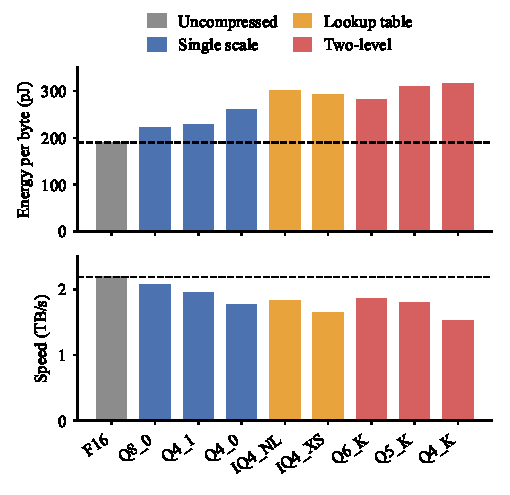
\includegraphics[width=\columnwidth]{energy.pdf}
\caption{Energy per byte (top) and speed (bottom) when multiplying a matrix stored in each format by a vector on
the H100. The dashed lines mark uncompressed F16.}
\label{fig:energy}
\end{figure}
To measure the cost of each format, we store the same large matrix in every format and repeatedly multiply it by a
vector on the H100, which is the main operation performed while generating text. During the run we read the GPU's
built-in energy meter and subtract the power the GPU draws when idle, so that only the energy spent on the work
itself is counted. Fig.~\ref{fig:energy} shows two quantities for each format. The top panel shows the energy spent
per byte of weights read. If memory traffic were the only cost, every format would sit at the same height as
uncompressed F16, because each byte would cost the same to fetch. Anything above the F16 line is therefore extra
energy spent on handling the format. The bottom panel shows the speed, that is, how many bytes of weights the GPU
gets through per second. F16 needs no decompression and runs close to the maximum speed of the memory. When a format
runs more slowly, the memory is not the bottleneck any more: the GPU is busy decompressing.

The figure and Table~\ref{tab:energy} lead to three observations. First, compression saves less energy than it
saves data. Every compressed format spends more energy per byte than F16, up to two thirds more, so a format that
makes the weights 3.6 times smaller reduces energy by only 2.2 times. Second, the extra cost grows with the
complexity of the format. Q4\_0, Q4\_K and IQ4\_NL all store exactly the same number of bytes per weight, yet Q4\_K
uses 21\% more energy than the simple Q4\_0. Since the data read is identical, this difference must come from the
work of decompressing, which supports H1. Third, the extra cost has two different causes. The two-level formats,
such as Q4\_K, are slower, so the GPU stays busy for longer for the same amount of data. The lookup-table formats
are about as fast as the simple formats but draw more power while they run.

If every format cost as little energy per byte as F16, the energy of these matrix multiplications would drop by up
to about a third. This is an optimistic upper bound. A more realistic target, bringing all formats down to the cost
of the simplest compressed format, would save 15--20\%.

\section{Challenges}
The SCITAS cluster does not allow the detailed profiling tools that would show exactly what the GPU does while
decompressing, so we have to infer this indirectly. The GPU's energy meter covers the whole board, including memory,
so we cannot separate memory energy from computation energy. Our hardware design and the H100 are built in different
technologies, so we can only compare relative costs.

\section{Update on the Plan}

\subsection{Team composition and priorities}
The team composition is unchanged. We will first finish the GPU measurements, then design the hardware unit, and
finally combine both into an estimate of the energy saved. We have dropped the simulation of Avant-Garde.

\subsection{Milestones}
Table~\ref{tab:milestones} lists our milestones.
\begin{center}\small
\captionof{table}{Planned milestones, with the week counted from the submission of this report.}
\label{tab:milestones}
\begin{tabular}{@{}lp{0.80\columnwidth}@{}}
\toprule
Week & Milestone\\
\midrule
1 & Energy measurements for all matrices of the model and for generating text with the full model\\
2 & Hardware unit for the single-scale and two-level formats\\
3 & Support for lookup-table formats; area and power estimates\\
4 & Energy comparison, final estimate and report\\
\bottomrule
\end{tabular}
\end{center}

\subsection{Final goal}
In the proposal, our goal was to compare how fast software and Avant-Garde handle compressed formats, using a
simulator. Our new goal has two parts. First, we want to measure how much energy a real GPU spends on decompressing
weights in software when running a local LLM. Second, we want to design a small hardware unit that extends
Avant-Garde to the formats used by GGUF and decompresses weights just before they are used, and to estimate how much
energy it saves per generated token and how much chip area and power it costs.

{\footnotesize
\begin{thebibliography}{9}\setlength{\itemsep}{0pt}
\bibitem{ag} M.~Gil et al., ``Avant-Garde: Empowering GPUs with Scaled Numeric Formats,'' ISCA, 2025.
\bibitem{splitwise} P.~Patel et al., ``Splitwise: Efficient Generative LLM Inference Using Phase Splitting,'' ISCA, 2024.
\bibitem{horowitz} M.~Horowitz, ``Computing's Energy Problem (and What We Can Do About It),'' ISSCC, 2014.
\bibitem{mxnpu} Z.~Zhao et al., ``MX-Like Tensor Core for LLM Inference with NPU Integration,'' arXiv:2610.26083, 2026.
\bibitem{lut} Z.~Mo et al., ``LUT Tensor Core: A Software-Hardware Co-Design for LUT-Based Low-Bit LLM Inference,'' ISCA, 2025.
\bibitem{flute} H.~Guo et al., ``Fast Matrix Multiplications for Lookup Table-Quantized LLMs,'' Findings of EMNLP, 2024.
\end{thebibliography}}
\end{document}
